% Constructed and checked from the problem; not a geometric proof.
\documentclass[tikz,border=8pt]{standalone}
\begin{document}
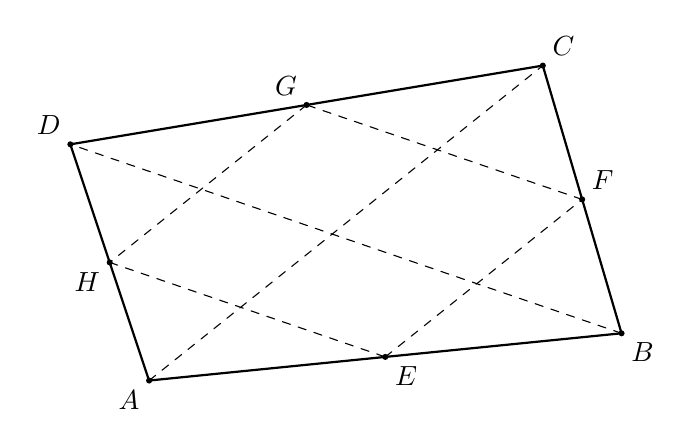
\begin{tikzpicture}[scale=1,line cap=round,line join=round]
\coordinate (p0) at (0,0);
\coordinate (p1) at (6,0.6);
\coordinate (p2) at (5,4);
\coordinate (p3) at (-1,3);
\coordinate (p4) at (3,0.3);
\coordinate (p5) at (5.5,2.3);
\coordinate (p6) at (2,3.5);
\coordinate (p7) at (-0.5,1.5);
\draw[thick] (p0) -- (p1);
\draw[thick] (p1) -- (p2);
\draw[thick] (p2) -- (p3);
\draw[thick] (p3) -- (p0);
\draw[dashed] (p0) -- (p2);
\draw[dashed] (p1) -- (p3);
\draw[dashed] (p4) -- (p5);
\draw[dashed] (p5) -- (p6);
\draw[dashed] (p6) -- (p7);
\draw[dashed] (p7) -- (p4);
\fill (p0) circle (1.1pt) node[below left] {$A$};
\fill (p1) circle (1.1pt) node[below right] {$B$};
\fill (p2) circle (1.1pt) node[above right] {$C$};
\fill (p3) circle (1.1pt) node[above left] {$D$};
\fill (p4) circle (1.1pt) node[below right] {$E$};
\fill (p5) circle (1.1pt) node[above right] {$F$};
\fill (p6) circle (1.1pt) node[above left] {$G$};
\fill (p7) circle (1.1pt) node[below left] {$H$};
\end{tikzpicture}
\end{document}
